\documentclass{beamer}

\mode<handout>{
  \usepackage{parskip}
}
\mode<beamer>{
  \usetheme{Rochester}
}
\usepackage{geometry}
\usepackage[utf8x]{inputenc}
\usepackage{tikz}
\usepackage{graphicx}
\usetikzlibrary{mindmap}
\usefonttheme{serif}
\usetikzlibrary{shapes.callouts}
\usepackage[T1]{fontenc}
\usepackage{lmodern}
\usepackage[underline=true,rounded corners=false]{pgf-umlsd}
\usepackage{tikz-uml}
\usepackage{url}
\usepackage{float}
\DeclareGraphicsRule{.tif}{png}{.png}{`convert #1 `dirname #1`/`basename #1 .tif`.png}

\setbeamertemplate{navigation symbols}{}

\newcommand{\green}[1]{\textcolor{green!50!black}{#1}}

\title{A Generalized Model for Peer Review:\\Design and Implementation}
\author{Xiang Gao}
\date{Dec 19, 2011}

\begin{document}

%----------- titlepage ----------------------------------------------%
\begin{frame}[plain]
  \titlepage
\end{frame}

%----------- slide --------------------------------------------------%
\begin{frame}
  \frametitle{Six Building Blocks for Modeling Peer Review}
\begin{center}
\resizebox{8cm}{!}{
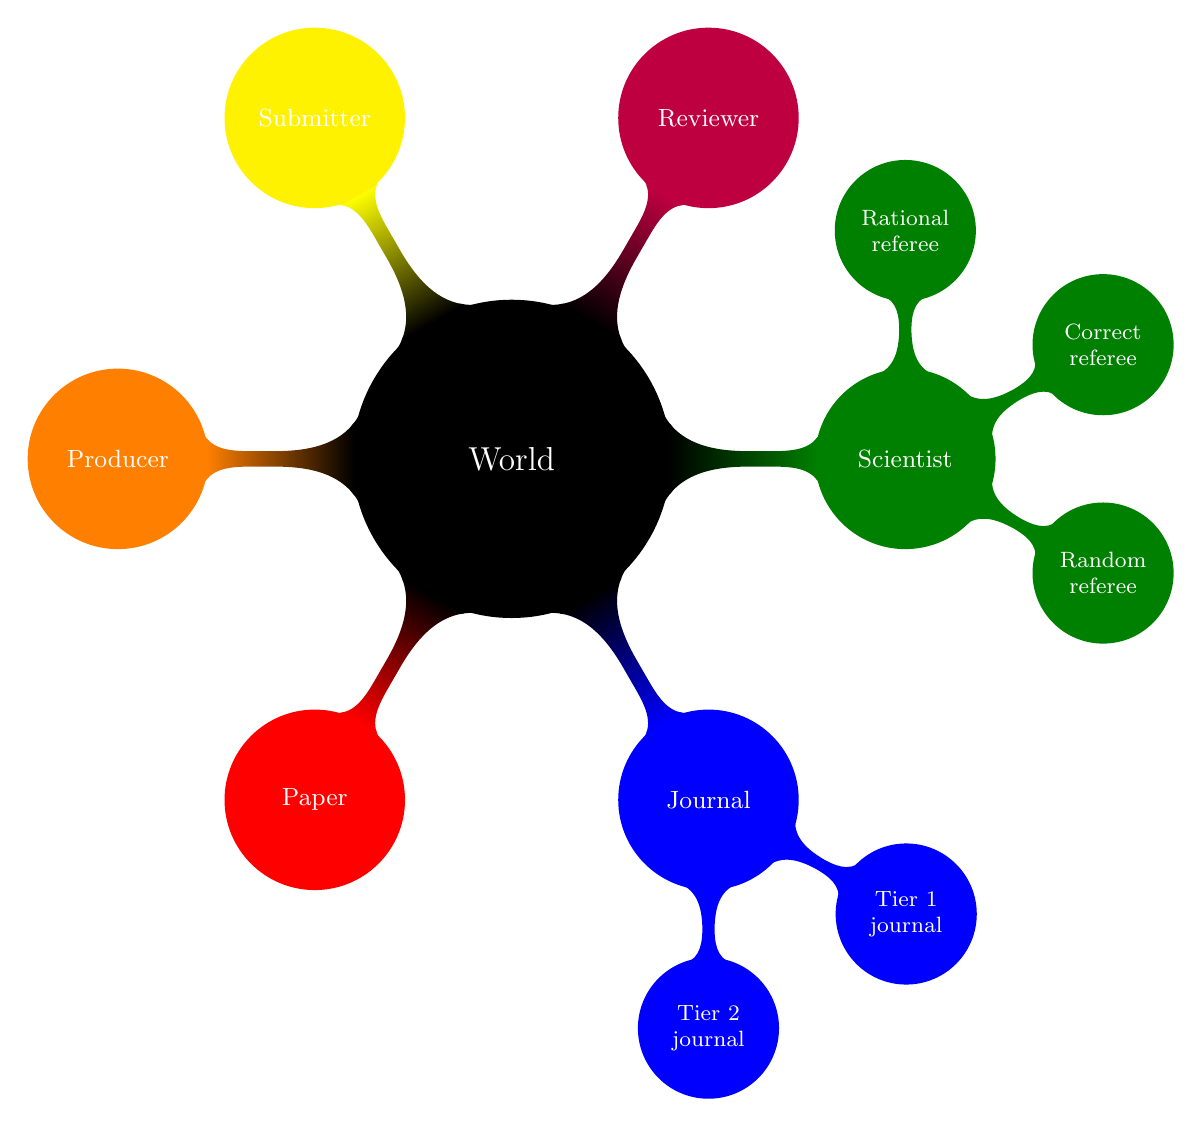
\begin{tikzpicture}[]
      \path[mindmap,concept color=black,text=white]
        node[concept] {World}
        [clockwise from=0]
        child[concept color=green!50!black] {
          node[concept] {Scientist}
          [clockwise from=90]
            child { node[concept] {Rational referee} }
            child { node[concept] {Correct referee} }
            child { node[concept] {Random referee} }
        }
        child[concept color=blue] {
        node[concept] {Journal}
        [clockwise from=-30]
          child { node[concept] {Tier 1 journal} }
          child { node[concept] {Tier 2 journal} }
        }
        child[concept color=red] { node[concept] {Paper} }
        child[concept color=orange] { node[concept] {Producer} }
        child[concept color=yellow] { node[concept] {Submitter} }
        child[concept color=purple] { node[concept] {Reviewer} };
    \end{tikzpicture}
    }
\end{center}
\end{frame}

%----------- slide --------------------------------------------------%
\begin{frame}
  \frametitle{Class Design}

\begin{center}
\begin{figure}
\resizebox{10cm}{!}{
\begin{tikzpicture}
\begin{umlpackage}{Common}
\umlclass{Scientist}{
  id  \\ intelligence
}{
  produce\_paper(Producer) : Paper\\
  submit\_paper(Submitter)
}

\umlclass[y=-3]{Paper}{
  id \\ quality
}{}

\umlclass[y=-7]{Journal}{
  id \\ impact
}{
  review\_paper(Reviewer)
}

\umlclass[x=5,y=-3.5]{World}{
  Scientist \\ Journal
}{
  simulate\_world(Simulator)
}

\umlinterface[x=5,y=-7]{Simulator}{}{
  simulate(World)
}

\umlinterface[x=10,y=0]{Producer}{}{
  produce(Scientist)
}

\umlinterface[x=10,y=-3]{Submitter}{}{
  submit(Paper)
}

\umlinterface[x=10,y=-7]{Reviewer}{}{
  review(Journal, Paper)
}

\umlunicompo{World}{Scientist}
\umlunicompo{World}{Journal}
\umlunicompo{World}{Paper}
\umlunicompo{World}{Producer}
\umlunicompo{World}{Submitter}
\umlunicompo{World}{Reviewer}
\umldep{World}{Simulator}

\end{umlpackage}
\end{tikzpicture}
}
\end{figure}
\end{center}
\end{frame}

%----------- slide --------------------------------------------------%
\begin{frame}
  \frametitle{Work Flow}
  
\begin{figure}
  \centering
  \resizebox{9cm}{!}{
  \begin{sequencediagram}
    \newthread{sci}{Scientist}
    \newinst{pro}{Producer}
    \newinst{pp}{Paper}
    \newinst{sub}{Submitter}
    \newinst{jor}{Journal}
    \newinst{rev}{Reviewer}

    \begin{sdloop}{Run Loop}
      \begin{call}{sci}{produce\_paper()}{pro}{paper}
        \begin{callself}{pro}{produce()}{}
        \end{callself}
      \end{call}
      \begin{call}{sci}{submit\_paper()}{sub}{journal}
        \begin{callself}{sub}{submit()}{}
        \end{callself}
      \end{call}
      \begin{call}{jor}{review\_paper()}{rev}{decision}
        \begin{callself}{rev}{review()}{}
        \end{callself}
      \end{call}
    \end{sdloop}
  \end{sequencediagram}
  }
\end{figure}

\end{frame}

%----------- slide --------------------------------------------------%
\begin{frame}
\frametitle{Code Style}

\begin{itemize}
  \item \large{Objected-oriented for extendibility.}
  \item \large{Comment to generate help doc.}
  \item \large{Parallel for simulation.}
\end{itemize}

\end{frame}

%----------- slide --------------------------------------------------%
\begin{frame}
\frametitle{Thurner's Model: Introduction}

\begin{block}{Model}
$Q_{i}^{author} \in N(100, \sigma^{2})$
\bigskip
$Q_{i}^{submit} \in N(Q_{i}^{author}, \sigma^{2}_{quality})$
\bigskip
$M(t) = \lambda M(t-1) + (1 - \lambda) \langle Q_{i}^{quality}(t-1)\rangle_{i}$
\bigskip
$Q_{min} = M(t) + \alpha std[Q_{i}^{quality}(t-1)]$
\end{block}

\end{frame}

%----------- slide --------------------------------------------------%
\begin{frame}
\frametitle{Thurner's Model: Results and Discussion}
\begin{figure}
    \begin{center}
    \resizebox{7cm}{!}{\includegraphics{../figure/Thurner/avg_quality_100_0_0.eps}}
    \caption{The average paper quality when all the reviewers are correct ones.}
    \end{center}
\end{figure}
\end{frame}

%----------- slide --------------------------------------------------%
\begin{frame}
\frametitle{Thurner's Model: Results and Discussion}
\begin{figure}
    \begin{center}
    \resizebox{7cm}{!}{\includegraphics{../figure/Thurner/avg_quality_90_0_10.eps}}
    \caption{The average paper quality when 90 percent the reviewers are correct ones and 10 percent are rational.}
    \end{center}
\end{figure}
\end{frame}

%----------- slide --------------------------------------------------%
\begin{frame}
\frametitle{Thurner's Model: Results and Discussion}
\begin{figure}
    \begin{center}
    \resizebox{7cm}{!}{\includegraphics{../figure/Thurner/no_network_comparison.eps}}
    \caption{Comparison of average paper quality when varying the fraction of random reviewers from 0 to 0.2, the fractional of rational reviewers from 0 to 0.7.}
    \end{center}
\end{figure}
\end{frame}

%----------- slide --------------------------------------------------%
\begin{frame}
\frametitle{Thurner's Model: Results and Discussion}
\begin{figure}
    \begin{center}
    \resizebox{7cm}{!}{\includegraphics{../figure/Thurner/network_comparison.eps}}
    \caption{Comparison of average paper quality of when 10 percent scientists are in network and varying the fractional of rational reviewers from 0 to 0.7.}
    \end{center}
\end{figure}
\end{frame}

%----------- slide --------------------------------------------------%
\begin{frame}
\frametitle{Thurner's Model: Results and Discussion}
\begin{figure}
    \begin{center}
    \resizebox{7cm}{!}{\includegraphics{../figure/Thurner/journal_comparison.eps}}
    \caption{Effect of journal favors higher quality papers.}
    \end{center}
\end{figure}
\end{frame}

%----------- slide --------------------------------------------------%
\begin{frame}
\frametitle{Thurner's Model: Results and Discussion}
\begin{figure}
    \begin{center}
    \resizebox{7cm}{!}{\includegraphics{../figure/Thurner/acc_num_100_0_0_0.eps}}
    \caption{Average accepted quality vs accepted numbers. The reviewers are all correct ones.}
    \end{center}
\end{figure}
\end{frame}

%----------- slide --------------------------------------------------%
\begin{frame}
\frametitle{Lessons and Experiences}
\begin{itemize}
  \item<1-> \large{Start early.}
  \item<2-> \large{Plan to throw one away.}
  \item<3-> \large{Don't repeat yourself.}
  \item<4-> \large{Summary and outlook.}
\end{itemize}
\end{frame}

\end{document}